\section{\textit{Simulador de Ambiente Virtual}}

\subsection{Apresentação e Resumo}

VRide é um jogo que deverá ser utilizado em uma plataforma de bicileta de realidade virtual para simular percursos de bicicleta em diferentes cenários.

\subsection{Principais Características}

\subsubsection{Simulação de Corrida}

O jogo é um simulador de corrida em bicicleta. Possuirá sistema de voltas, podendo escolher o número de voltas na pista e ter o tempo das voltas medido e armazenado para efeitos de comparação futura.

\subsubsection{Conta de Usuário}

O jogador poderá criar contas locais para guardar preferências, recordes e dados de desempenho coletados pelo subsistema eletrônico. O jogo apresentará gráficos apresentando a evolução desses indicadores.

\subsubsection{Dois tipos de pista}

Haverá dois tipos de pista. Uma será baseada em circuitos de corrida \textit{indoor} e é focada em treinos profissionais e evolução do usuário em relação aos exercícios. A segunda será baseada em cenários abertos comumente usados para ciclismo como parques e bosques. Nesse tipo de pista o foco será na exploração do ambiente e experimentação das diferentes sensações de elevação e vibração proporcionadas pelo projeto.

\subsection{Público-Alvo}

O jogo será feito para os usuários do laboratório da bicicleta de realidade virtual localizado no campus Gama da UnB.

\subsection{Plataformas}

O jogo será desenvolvido para computadores e poderá ser executado nos sistemas operacionais \textit{Windows} e \textit{Linux}.

\subsection{Controles}

\begin{itemize}
\item Giroscópio do \textit{oculus}: selecionar opções do jogo.
\item Botão integrado na estrutura: pausar o jogo.
\end{itemize}

\subsection{Interfaces}

A tela inicial do jogo apresentará duas modalidades de jogo: pista lisa ou pista com irregularidades. Cada modalidade de jogo possuirá um cenário diferente.

Ao final do jogo, serão apresentadas informações de desempenho do jogador durante o percurso.

\subsection{Unity 3D}

A \textit{engine} Unity 3D será utilizada para a construção dos menus e cenários. Ela é uma \textit{engine} comumente utilizada para a criação de jogos e foi escolhida como ferramenta pela integração com o óculos de realidade virtual e ferramentas de criação de ambientes 3D interativos. Possui uma arquitetura baseada em componentes e suas linguagens de programação padrão são C\# e Javascript.

\subsection{Oculus SDK}

\begin{center}
	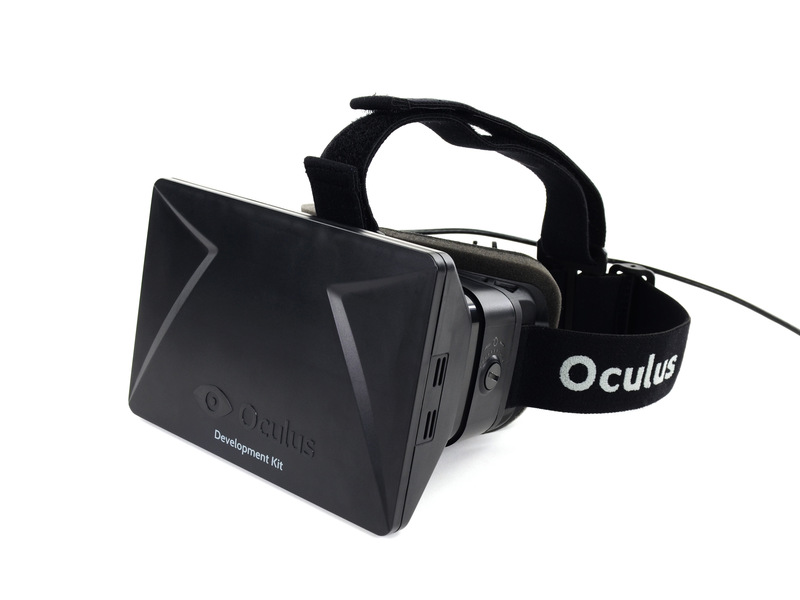
\includegraphics[scale=0.4]{figuras/Oculos_sdk}
	\captionof{figure}{Modelo de óculos \textit{rift} disponível para o projeto.}
\end{center} 

O Oculus SDK é o kit de desenvolvimento a ser utilizado para a criação do ambiente de realidade virtual. Será utilizada a versão DK1 disponibilizada
pelos patrocinadores do projeto. O kit inclui um óculos de realidade virtual com os componentes necessários para conectá-lo com um computador com placa gráfica, ponto necessário para a construção do sistema.

\subsection{Testes}

Os testes serão realizados na ferramenta \textit{Unity Test Runner} disponibilizada pelo \textit{Unity 3D}. Essa ferramenta permite que os testes sejam executados tanto em \textit{Edit Mode} quanto em \textit{Play Mode}.

\section{\textit{Sistemas de Aquisição e Controle}}

\subsection{Apresentação e Resumo}
Todos os subsistemas propostos são feitos para mensurar dados fisiológicos e de desempenho para um futuro feedback para o atleta e controlar os atuadores presentes na plataforma.

\subsection{Principais Características}

\subsubsection{Monitoramento da Bicicleta}
O monitoramento da bicicleta se dá através de sensores de velocidade e aceleração, considerando passar estes parâmetros para o jogo de realidade virtual, possibilitando uma maior inserção do usuário no ambiente. O  sistema será feito também de encoders, afim de que consigamos mensurar a distância percorrida pelo atleta, guardando este dado para que na posteridade possamos analisar com dados de outras sessões (indoor) ou até mesmo com dados cruzados em atividades externas (outdoor). Ademais este sistema também será responsável por captar dados referentes ao movimento angular do guidão, acionamento dos freios e deteção de presença do usuário assim que este se sentar na bicicleta. 

\subsubsection{Monitoramento do Atleta}

O sistema principal a ser desenvolvido. Este subsistema tem como escopo mensurar dados fisiológicos do usuário, como batimento cardíaco, resistência na palma da mão e também fazer uma estimativa da respiração do usuário com o intuito de gerar parâmetros para análise sobre a diferença na prática de esportes no ambiente virtual e no real. 

\subsubsection{Controle de atuadores}
Eles são responsáveis por agregar a sensação de movimento à plataforma da bicicleta, simulando os ambientes de inclinação, ladeiras e declives, concomitante ao ambiente virtual reproduzido nos óculos. Para emular os níveis de aceleração de aclives e declives serão utilizado motores e/ou geradores elétricos. Os algoritmos são escopos do projeto.

\subsubsection{Comunicação dos módulos}
Os subsistemas acima supracitados fornecem parâmetros que podem ser vistos pelos usuários. Estes parâmetros serão passados para a interface gráfica, disponível no óculos. A parte de comunicação entre os módulos e o óculos será desenvolvida pela equipe de eletrônica conjunto a equipe de software.

\subsection{Testes}
Os testes serão feitos de acordo com cronograma disposto, comparando os dados adquiridos com os resultados desenvolvidos em pesquisas e artigos científicos já disponibilizados em bases de consulta. Para validação dos sistemas finais, os sistemas deverão responder a um nível satisfatório ao serem comparados com equipamentos profissionais, caso haja possibilidade de usufruir destas ferramentas.

\section{\textit{Estrutura}}

\subsection{Apresentação e Resumo}
Desenvolvimento de uma plataforma física com intuito de acoplar todos os outros sistemas desenvolvidos: sensores, atuadores, entre outros e concluir um sistema de segurança com o objetivo de preservar a integridade física do usuário.

\begin{center}
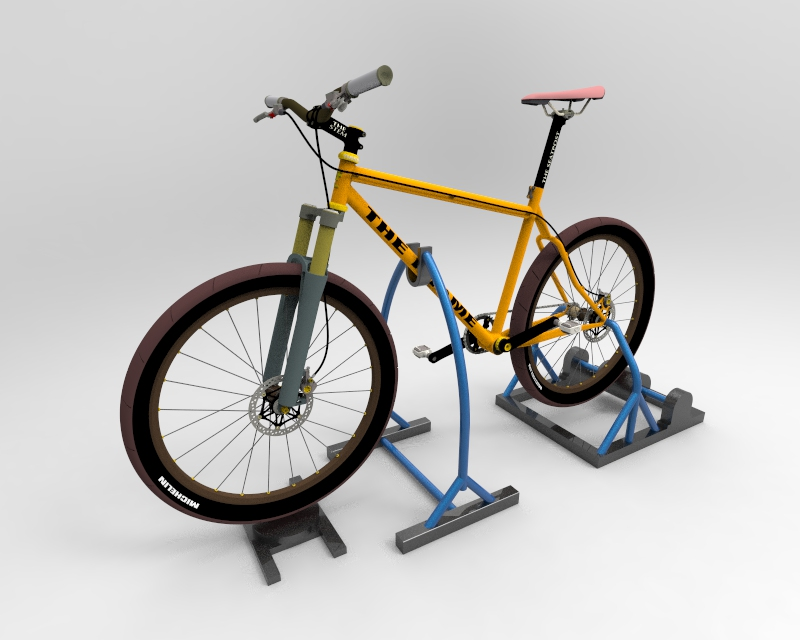
\includegraphics[scale=0.4]{figuras/bike_1}
	\captionof{figure}{Modelo de bicileta acoplada a estrutura proposta.}
\end{center} 

\subsection{Principais Características}
\subsubsection{Desenvolvimento da plataforma}
Visa o desenvolvimento de uma plataforma para acoplamento da bicicleta da maneira mais simples possível. Isto envolve todo dimensionamento da parte modular e posicionamento dos componentes dos sistemas. O projeto deste subsistema deve ser todo simulado de forma computacional, para melhor avaliação dos materiais a serem escolhidos, peso e esforços na plataforma.

\subsubsection{Segurança}
Como o ambiente virtual junto com a utilização da plataforma (caracterizando uma realidade aumentada) pode gerar um certo desconforto para o usuário, é proposto pela equipe um sistema que auxilie o usuário em momentos de dificuldade ou que possam acarretar em acidentes. Para tal, haverá toda a documentação e estudo quanto a melhor disposição dos equipamentos de segurança.

\begin{center}
	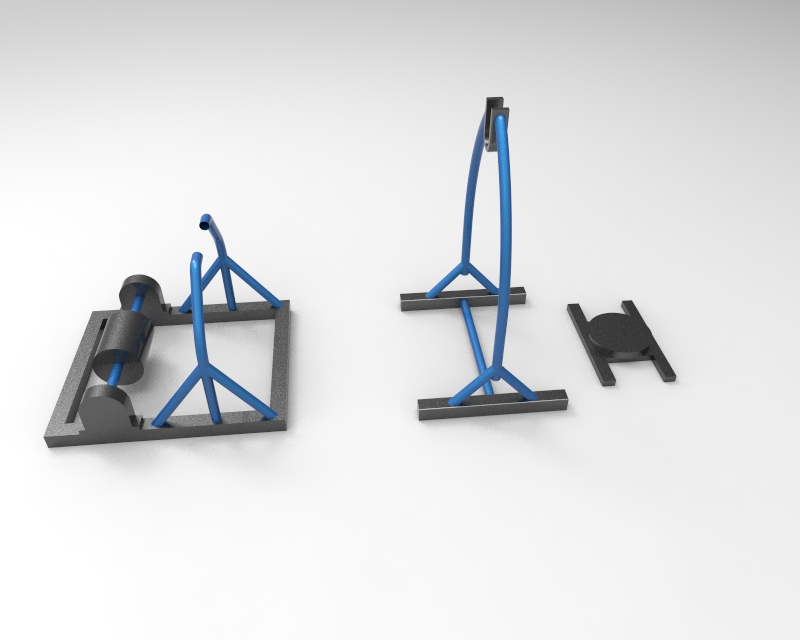
\includegraphics[scale=0.4]{figuras/bike_2}
	\captionof{figure}{Versão inicial da estrutura de acoplamento da bicleta.}
\end{center} 

\subsection{Testes}
Os testes serão feitos por meio de análises computacionais, utilizando os softwares CATIA V5R19 e Ansys 17.2. A cada modificação do Design será feito análises tanto estáticas quanto dinâmicas para garantir que a estrutura seja bem firme e aguente bem mais que os esforços e excitações causados pelos equipamentos e pelo usuário.

\section{\textit{Sistemas de Alimentação de Energia }}
\subsection{Apresentação e Resumo}
O subsistema de alimentação visa identificar as principais formas de alimentação energética do projeto. Ou seja, o subsistema é responsável por identificar os gastos energéticos oriundos de todos os subsistemas que compõem o produto em sua totalidade, bem como formular e executar um sistema de geração de energia, seja ele autônomo ou não,  a fim de satisfazer as necessidades criadas e promover a integração entre todos os subsistemas da plataforma.  

Para tanto, as principais tarefas que o subgrupo se concentrará em realizar são listadas e descritas a seguir.

\subsection{Principais Características}
\subsubsection{Atuadores da plataforma}
	Dimensionar os motores a serem utilizados para realizar o movimento da estrutura. De acordo com a delimitação dos movimentos que a bicicleta terá que realizar para atender o escopo da estrutura do projeto serão dimensionados motores que permitam a execução das tarefas demandadas, inicialmente prevê-se a solução de utilizar um alternador como gerador a fim de utilizar a corrente que sairá deste para atribuir diferentes dificuldades nas pedaladas que o usuário realizará, através de um sistema de controle que com a variação desta dista corrente permita simular diferentes cenários de dificuldade de acordo com a realidade virtual correspondente. 	

\subsubsection{Estudo energético do sistema}
Serão mapeados todos os equipamentos do projeto que consomem energia durante seu funcionamento e seus respectivos consumos serão quantificado em unidade de potência (W) através da ficha técnica e cálculos periódicos de consumo (por hora, por dia, por mês, etc).

\subsubsection{Sistema de alimentação energética} Através do mapeamento do consumo energético do sistema serão realizadas propostas de formas de alimentação para este sistema através da seleção de baterias ou geradores ou ainda, através da rede elétrica convencional de energia integradas a contribuição da energia a ser gerada pelo próprio sistema. 
 
\subsubsection{Conversão de energia}Realizar a conversão da energia mecânica gerada pelas pedaladas no equipamento em energia elétrica. A bicicleta será acoplada a uma estrutura fixa onde sua roda será posicionada em uma espécie de rolo de treino, neste rolo de treino será acoplado um alternador a fim de converter a energia mecânica oriunda das pedaladas em energia elétrica.

\subsubsection{Armazenamento da energia elétrica} O alternador citado anteriormente terá duas saídas, além de fornecer energia que será utilizada para dificultar o movimento de pedaladas em cenários de inclinação, fornecerá energia (que após retificada) será direcionada a uma bateria que será responsável por armazenar esta energia gerada, esta bateria possuirá tensão de 12V, assim sendo, que será utilizada para alimentar dispositivos menos exigentes tais como sensores e carregar componentes como o óculos e computadores. 

\subsection{Testes}
Os testes serão feitos concomitantemente aos sistemas de controle dos atuadores, descritos no sistema de aquisição e controle.